% ============================================================
%  DIABETES_REIMPLEMENTATION_SLIDES.tex
%  Slide version of DIABETES_REIMPLEMENTATION_REPORT_v2: what the baseline
%  paper did, what the repository audit did, what the re-implementation did,
%  how they compare, and the remaining gaps with fixes.
%  All tables are \input from reimplementation/tex/slides/ (generated by
%  build_slide_tables.py); figures from reimplementation/figures/.
%  Compile: tectonic DIABETES_REIMPLEMENTATION_SLIDES.tex
% ============================================================
\documentclass[aspectratio=169,10pt,t,xcolor={table}]{beamer}
\usetheme{Madrid}
\usepackage{amsmath,amssymb}
\usepackage{booktabs,array}
\usepackage{graphicx}
\usepackage{tikz}
\usetikzlibrary{positioning,arrows.meta,calc,fit}
\graphicspath{{../reimplementation/figures/}}
\newcommand{\tabdir}{../reimplementation/tex/slides/}

\definecolor{qnavy}{HTML}{1B3A5C}
\definecolor{qteal}{HTML}{0E7C7B}
\definecolor{qred}{HTML}{B23A3A}
\definecolor{qgreen}{HTML}{2E7D4F}
\definecolor{qamber}{HTML}{C9821B}
\definecolor{qlight}{HTML}{EEF3F8}
\setbeamercolor{structure}{fg=qnavy}
\setbeamercolor{palette primary}{bg=qnavy,fg=white}
\setbeamercolor{palette secondary}{bg=qteal,fg=white}
\setbeamercolor{palette tertiary}{bg=qnavy,fg=white}
\setbeamercolor{frametitle}{bg=qnavy,fg=white}
\setbeamercolor{title}{bg=qnavy,fg=white}
\setbeamercolor{block title}{bg=qnavy,fg=white}
\setbeamercolor{block body}{bg=qlight,fg=black}
\setbeamercolor{block title alerted}{bg=qred,fg=white}
\setbeamercolor{block body alerted}{bg=qred!7,fg=black}
\setbeamercolor{block title example}{bg=qteal,fg=white}
\setbeamercolor{block body example}{bg=qteal!8,fg=black}
\setbeamercolor{item}{fg=qteal}
\setbeamertemplate{navigation symbols}{}
\setbeamertemplate{itemize items}[circle]
\setbeamertemplate{enumerate items}[default]
\setbeamerfont{frametitle}{size=\large,series=\bfseries}
\setbeamertemplate{caption}{\raggedright\insertcaption\par}
\setbeamertemplate{section page}{%
  \begin{centering}\vspace{2.6cm}
  {\usebeamercolor[fg]{structure}\LARGE\bfseries\insertsection\par}
  \end{centering}}
\AtBeginSection{\frame[plain]{\sectionpage}}

\newcommand{\ok}[1]{\textcolor{qgreen}{\textbf{#1}}}
\newcommand{\bad}[1]{\textcolor{qred}{\textbf{#1}}}
\newcommand{\warn}[1]{\textcolor{qamber}{\textbf{#1}}}
\newcommand{\code}[1]{\texttt{\small #1}}
\newcommand{\src}[1]{{\tiny\textcolor{gray}{Source: #1}}}

\title[Daga et al.\ (2026) on Diabetes: re-implementation and verification]{Daga et al.\ (2026) on the Pima Indians Diabetes dataset}
\subtitle{What the paper did, what the repository audit did, what the independent re-implementation found, and the gaps that remain}
\author[M.~Wajahat]{Prepared for M.~Wajahat}
\institute[]{Repository \texttt{Adaptive-Quantum-Kernel-Selection}, code in \texttt{reimplementation/}}
\date{19 October 2026}

\begin{document}

\begin{frame}[plain]
\titlepage
\end{frame}

\begin{frame}{Roadmap}
\begin{columns}[T]
\column{0.55\textwidth}
\begin{enumerate}
  \item \textbf{The baseline paper}: what Daga et al.\ (2026) built, claimed and measured.
  \item \textbf{What the repository audit did before}: the IEEE manuscript (v1--v3) and the comparison reports.
  \item \textbf{The re-implementation}: rules, pipeline, kernels, audit extensions, cross-checks.
  \item \textbf{Paper vs re-implementation}: every published Diabetes table side by side.
  \item \textbf{Beyond the paper}: seeds, family-wise correction, fold-local preprocessing, model selection, tuned baselines.
  \item \textbf{Gaps and fixes}: in the paper, in the audit, in the re-implementation.
\end{enumerate}
\column{0.42\textwidth}
\begin{block}{One-line answer}
The paper's Diabetes numbers reproduce to the last digit (108/108 bootstrap values). The \emph{interpretation} changes: the recall gain is real, the accuracy advantage is not, the VQC is untrained, and the noise baseline is the wrong circuit.
\end{block}
\begin{exampleblock}{Reading guide}
\ok{green} = reproduces / passes; \warn{amber} = explained difference; \bad{red} = does not hold.
\end{exampleblock}
\end{columns}
\end{frame}

% ============================================================
\section{Part 1: What the baseline paper did}
% ============================================================

\begin{frame}{The proposal: three quantum kernels, two classifiers, one meta-learner}
\begin{center}
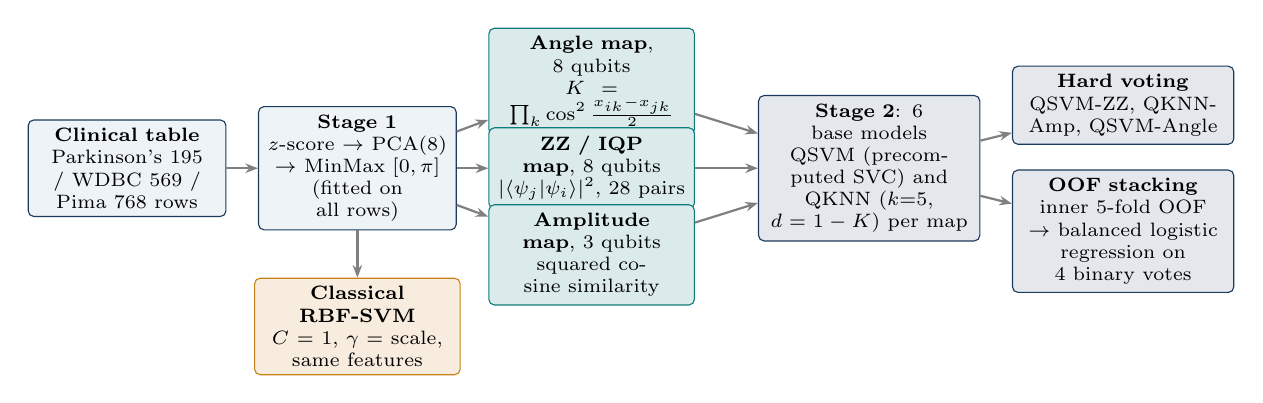
\begin{tikzpicture}[font=\scriptsize, node distance=4mm,
  box/.style={draw, rounded corners=2pt, align=center, inner sep=3pt, minimum height=8mm},
  d/.style={box, fill=qlight, draw=qnavy, text width=2.3cm},
  q/.style={box, fill=qteal!15, draw=qteal, text width=2.4cm},
  c/.style={box, fill=qamber!15, draw=qamber, text width=2.4cm},
  e/.style={box, fill=qnavy!12, draw=qnavy, text width=2.6cm},
  arr/.style={-{Stealth[length=1.6mm]}, thick, gray}]
\node[d] (data) {\textbf{Clinical table}\\Parkinson's 195 / WDBC 569 / Pima 768 rows};
\node[d, right=of data] (prep) {\textbf{Stage 1}\\$z$-score $\to$ PCA(8) $\to$ MinMax $[0,\pi]$\\(fitted on all rows)};
\node[q, right=of prep, yshift=11mm] (ang) {\textbf{Angle map}, 8 qubits\\$K=\prod_k\cos^2\frac{x_{ik}-x_{jk}}{2}$};
\node[q, right=of prep] (zz) {\textbf{ZZ / IQP map}, 8 qubits\\$|\langle\psi_j|\psi_i\rangle|^2$, 28 pairs};
\node[q, right=of prep, yshift=-11mm] (amp) {\textbf{Amplitude map}, 3 qubits\\squared cosine similarity};
\node[e, right=of zz, xshift=4mm] (base) {\textbf{Stage 2}: 6 base models\\QSVM (precomputed SVC) and\\QKNN ($k{=}5$, $d=1-K$) per map};
\node[e, right=of base, yshift=8mm] (hv) {\textbf{Hard voting}\\QSVM-ZZ, QKNN-Amp, QSVM-Angle};
\node[e, right=of base, yshift=-8mm] (st) {\textbf{OOF stacking}\\inner 5-fold OOF $\to$ balanced logistic regression on 4 binary votes};
\node[c, below=of prep, yshift=-2mm] (rbf) {\textbf{Classical RBF-SVM}\\$C=1$, $\gamma=$ scale, same features};
\draw[arr] (data) -- (prep);
\draw[arr] (prep) -- (ang); \draw[arr] (prep) -- (zz); \draw[arr] (prep) -- (amp);
\draw[arr] (ang) -- (base); \draw[arr] (zz) -- (base); \draw[arr] (amp) -- (base);
\draw[arr] (base) -- (hv); \draw[arr] (base) -- (st);
\draw[arr] (prep) -- (rbf);
\end{tikzpicture}
\end{center}
\begin{itemize}
  \item Evaluation: stratified 10-fold CV (seed 42), metrics on pooled out-of-fold predictions, 1,000 stratified bootstrap resamples for means and 95\,\% intervals, paired bootstrap $p$-values against the RBF-SVM; also fold-level $t$-tests and McNemar tests.
  \item Extras: ablation, classical ensembles (XGBoost, Random Forest, SVM+KNN stacker), calibration (ECE, Brier, Platt), SHAP/LIME/permutation, PCA ``biomarker backtracking'', depolarizing-noise study, and a variational quantum classifier (VQC) as a negative baseline.
\end{itemize}
\end{frame}

\begin{frame}{What the paper claims (as printed)}
\begin{columns}[T]
\column{0.5\textwidth}
\begin{block}{Headline claims across the three datasets}
\tiny
\begin{tabular}{llcc}
\toprule
Dataset & Headline metric & RBF-SVM & Quantum stacking \\
\midrule
Parkinson's & Specificity & 0.585 & \textbf{0.813} ($p<0.001$) \\
Breast cancer & Specificity & 0.948 & 0.943 (n.s.) \\
Diabetes & Recall & 0.553 & \textbf{0.621} ($p=0.004$) \\
\bottomrule
\end{tabular}
\par\medskip\footnotesize
``Adaptive'' kernel selection: the meta-learner weights the base models per dataset; ``leakage-free'': stacking features are out-of-fold.
\end{block}
\column{0.47\textwidth}
\begin{block}{Diabetes is the paper's ``noise stress-test''}
\begin{itemize}\scriptsize
  \item Weak class separability; no model above 0.77 accuracy.
  \item Stacking has the highest accuracy (0.766) and recall (0.621): ``6.8 percentage points, roughly 24 additional diabetic patients per 1,000 screened''.
  \item Price: specificity 0.844 vs 0.867 for RBF; explained by the balanced class weight.
  \item QKNN-Amplitude ``collapses'' (0.711) and receives a negative coefficient ($-0.353$): presented as the ensemble's ``core safety mechanism''.
  \item VQC fails (0.540), attributed to a barren plateau.
  \item Under 10\,\% depolarizing noise the ensemble degrades most on Diabetes ($+0.083$ accuracy, $+0.125$ specificity).
\end{itemize}
\end{block}
\end{columns}
\src{Daga et al., Sci.\ Rep.\ 16:26840, pages 18--28; values transcribed from the PDF.}
\end{frame}

\begin{frame}{The paper's Diabetes results table (Table 9, as published)}
\begin{center}
{\scriptsize\input{\tabdir pub_table9.tex}}
\end{center}
\begin{itemize}\footnotesize
  \item 1,000-iteration stratified bootstrap of the pooled 10-fold out-of-fold predictions; mean and 2.5/97.5 percentiles.
  \item Positive class = diabetic (268 of 768). Recall = diabetic detection rate; specificity = non-diabetic detection rate.
  \item The paper also reports: Table 10 (AUCs), 11 (ablation), 12 (McNemar), 13 (classical ensembles), 14--15 (calibration), 16--18 (explainability and biomarkers), 19 (noise) and Fig.~8 (VQC learning curve).
\end{itemize}
\end{frame}

% ============================================================
\section{Part 2: What the repository audit did before this work}
% ============================================================

\begin{frame}{The existing audit: WDBC and WBCO, not Diabetes}
\begin{columns}[T]
\column{0.5\textwidth}
\begin{block}{IEEE manuscript, versions 1--3 (\texttt{latex\_report/})}
\begin{itemize}\footnotesize
  \item Scope: WDBC ($N=569$) reproduced from the released code and cached Gram matrices; replicated on WBCO ($N=683$). Parkinson's and Diabetes declared out of scope.
  \item Findings: RBF-SVM equals or beats stacking in all 20 WDBC+WBCO seeds; no quantum-superior Holm survivor; fold-local TOST equivalence; QSVM-Angle omitted from the quartet; noise circuits differ from the benchmarked ones; VQC loss has zero gradient.
  \item v1$\to$v3 corrections: ``trace collapse'' retracted; the WBCO QKNN-Angle recall survivor shown to be a $B{=}1{,}000$ seed artefact.
\end{itemize}
\end{block}
\column{0.47\textwidth}
\begin{block}{Comparison and focus reports (October 2026)}
\begin{itemize}\footnotesize
  \item \emph{Comparison report v2}: six related QML papers checked against their own printed matrices; Daga et al.\ used only as a cross-paper reference.
  \item \emph{Daga-focus report and slides}: 13 gaps in Daga et al.\ listed from the text (subject leakage on Parkinson's, VQC protocol, Table-13 classical stacker, PCA backtracking, no FWER control, title says NISQ hardware); Diabetes numbers transcribed, not re-run.
\end{itemize}
\end{block}
\begin{alertblock}{Gap this work closes}
\footnotesize Nothing in the repository had executed the pipeline on Diabetes or tested the headline recall claim. This deck reports the first independent run.
\end{alertblock}
\end{columns}
\end{frame}

% ============================================================
\section{Part 3: What the re-implementation did}
% ============================================================

\begin{frame}{Rules of the re-implementation}
\begin{columns}[T]
\column{0.5\textwidth}
\begin{block}{Independence}
\begin{itemize}\footnotesize
  \item Written from the paper's text (\code{qks\_common.py}, 4 runner scripts). No code imported from the released \code{quantum\_clinical\_github.py}.
  \item The released script was read only to settle four ambiguities in the paper text (next slides).
  \item Dataset: Pima Indians Diabetes from the public UCI mirror; verified identical to OpenML \code{diabetes} v1 (768 rows, 268 positives).
\end{itemize}
\end{block}
\begin{block}{Environment}
\footnotesize Python 3.11.9, PennyLane 0.44.1 (\code{default.qubit}, \code{default.mixed}, \code{lightning.qubit}), scikit-learn 1.5.2, XGBoost 3.2.0 (CPU), statsmodels 0.14.4; Intel i7-10700, 16\,GB. The paper: Python 3.12 on Kaggle with \code{lightning.qubit/gpu} and GPU XGBoost.
\end{block}
\column{0.47\textwidth}
\begin{block}{What was run (Diabetes only, as requested)}
\begin{itemize}\footnotesize
  \item \code{run\_paper\_reproduction.py}: paper Tables 4--6, 9--18.
  \item \code{run\_noise.py}: Table 19 under three protocols.
  \item \code{run\_vqc\_curves.py}: Fig.~8.
  \item \code{run\_audit\_extensions.py}, \code{run\_fold\_local\_metrics.py}, \code{run\_vqc\_gradient\_check.py}: the audit extensions.
  \item \code{verify\_independent.py}: eight cross-checks against transcription errors, shared bugs and coincidence.
  \item \code{compare\_published.py}, \code{make\_figures.py}, \code{build\_slide\_tables.py}: every table and figure in this deck.
\end{itemize}
\end{block}
\end{columns}
\end{frame}

\begin{frame}{Pipeline walkthrough (what each step does)}
\begin{enumerate}\footnotesize
  \item \textbf{Input}: $\mathbf{X}\in\mathbb{R}^{768\times8}$ (Pregnancies, Glucose, BloodPressure, SkinThickness, Insulin, BMI, DiabetesPedigreeFunction, Age); $y=1$ for 268 diabetic patients.
  \item \textbf{Stage 1 preprocessing}: $z$-score, PCA to 8 components (seed 42), MinMax to $[0,\pi]$; fitted on all 768 rows as in the released code. With 8 attributes the PCA is a rotation (100\,\% variance).
  \item \textbf{Stage 2 kernels}: three $768\times768$ Gram matrices $K_{ij}=|\langle\psi(\mathbf{x}_j)|\psi(\mathbf{x}_i)\rangle|^2$ (Angle, ZZ/IQP, Amplitude), computed in closed form or from the statevector and checked against the PennyLane circuit (embedding, adjoint embedding, probability of $|0\rangle^{\otimes n}$).
  \item \textbf{Base models}: stratified 10-fold split (seed 42). RBF-SVM on the scaled features; QSVM = precomputed-kernel SVC on $K[\mathrm{tr},\mathrm{tr}]$ and $K[\mathrm{te},\mathrm{tr}]$; QKNN = 5-NN on $\max(0,1-K)$.
  \item \textbf{Ensembles}: hard voting of QSVM-ZZ, QKNN-Amp, QSVM-Angle. Stacking: inside each training fold an inner 5-fold loop (seed 42) gives out-of-fold \emph{binary} predictions of the quartet (QSVM-Amp, QKNN-Amp, QSVM-ZZ, QKNN-Angle); a balanced logistic regression is fitted on them and applied to the quartet's test-fold predictions.
  \item \textbf{Statistics}: metrics on pooled out-of-fold predictions; bootstrap with \code{np.random.seed(42)} and 1,000 stratified \code{resample} calls; two-sided $p=2\min\{P(\Delta\le0),P(\Delta\ge0)\}$ vs RBF; fold-level $t$-tests; exact McNemar below 25 discordant pairs.
  \item \textbf{Everything else} (ablation, classical baselines, calibration, SHAP/LIME/permutation, backtracking, noise, VQC) reuses the same folds and Gram matrices with the paper's stated settings.
\end{enumerate}
\end{frame}

\begin{frame}{Kernels: formulas, circuits and verification}
\begin{columns}[T]
\column{0.52\textwidth}
\begin{block}{Closed forms used (and checked against the circuits)}
\footnotesize
\begin{align*}
K_{\mathrm{Angle}}(\mathbf{x}_i,\mathbf{x}_j) &= \prod_{k=1}^{8}\cos^2\!\Big(\tfrac{x_{ik}-x_{jk}}{2}\Big) \\
K_{\mathrm{Amp}}(\mathbf{x}_i,\mathbf{x}_j) &= \frac{(\mathbf{x}_i^{\top}\mathbf{x}_j)^2}{\|\mathbf{x}_i\|^2\|\mathbf{x}_j\|^2} \\
K_{ZZ}(\mathbf{x}_i,\mathbf{x}_j) &= |\langle\psi(\mathbf{x}_j)|\psi(\mathbf{x}_i)\rangle|^2,\;\; |\psi(\mathbf{x})\rangle=\mathrm{IQP}(\mathbf{x})|0\rangle^{\otimes 8}
\end{align*}
IQP: Hadamards, $R_z(x_k)$, then $e^{-i x_k x_l Z_kZ_l/2}$ on all 28 pairs.
\end{block}
\column{0.45\textwidth}
\begin{exampleblock}{Verification}
\begin{itemize}\footnotesize
  \item Circuit value $P(|0\rangle^{\otimes n})$ vs closed form: max difference $9\times10^{-16}$ (Angle), $2\times10^{-16}$ (ZZ), $9\times10^{-16}$ (Amplitude) on 100 random pairs; $\le 1.6\times10^{-15}$ on 600 more pairs and a full row.
  \item Gram matrices symmetric, unit diagonal, positive semi-definite.
  \item Timing: 295,296 pairs per kernel, seconds in closed form; the circuit form would take hours.
\end{itemize}
\end{exampleblock}
\end{columns}
\end{frame}

\begin{frame}{Where the paper's text and the released code disagree}
\begin{block}{Four decisions; in each case the released behaviour was reproduced, because that is what produced the published tables}
\begin{enumerate}\footnotesize
  \item \textbf{Angle-map rotation axis.} Eq.~(3) and Table~6 say $R_y$; the released kernel uses \code{AngleEmbedding} with its default $R_x$. Noiseless \emph{and} depolarized kernels are identical either way (verified to $2\times10^{-16}$): \ok{no numerical effect}.
  \item \textbf{ZZ-map connectivity.} Eq.~(5) writes nearest-neighbour pairs; the released clean kernel uses \code{IQPEmbedding} with all 28 pairs. The released \emph{noise} experiment implements the 7-edge chain. So Tables 9--18 come from an all-to-all kernel and Table 19 from a chain kernel: \warn{large effect on the 0\,\% noise row}.
  \item \textbf{VQC protocol.} Fig.~8 uses an 80/20 split with 30 epochs; Tables 9 and 12 use the VQC inside the 10-fold loop with 15 in-fold epochs. Both are in the code.
  \item \textbf{Noise baseline.} The noise code evaluates the chain circuit at every level, including 0\,\%, so the ``clean'' row of Table 19 is not the benchmark kernel of Table 9.
\end{enumerate}
\end{block}
\end{frame}

\begin{frame}{Audit extensions applied to Diabetes (each answers one question)}
\tiny
\begin{tabular}{p{2.9cm}p{4.8cm}p{5.5cm}}
\toprule
Analysis & Question about the published result & Definition used here \\
\midrule
Multi-seed robustness & Is the seed-42 ranking an accident of one partition? & Whole pipeline repeated for seeds 0,1,2,3,4,5,10,42,100,999 (inner CV seed = outer seed; also the released convention, inner seed fixed at 42). \\
Holm correction & 36 uncorrected $p$-values are reported; what survives family-wise control? & 8 models $\times$ 4 metrics vs RBF = 32 hypotheses; stratified bootstrap $B=10{,}000$, $+1$-corrected $p$; Holm at $\alpha=0.05$. Also the released $B=1{,}000$ formula and the paper's parametric $t$-tests. \\
Fold-local preprocessing & Scaler/PCA/MinMax are fitted on all patients; does fitting them inside the training fold change anything? & \emph{Outer-fold-local}: refit per outer fold, kernels recomputed. \emph{Strictly nested}: also refit inside every inner fold. TOST ($\pm0.01$), paired bootstrap CI, McNemar. \\
Nested model selection & The quartet was fixed by hand; what would a data-driven choice pick? & All $\binom{6}{4}=15$ quartets scored inside each training fold by inner accuracy, balanced accuracy or meta-learner CV; winner stacked and tested. \\
Baseline fairness & Classical baselines use defaults; does tuning change the comparison? & Nested \code{GridSearchCV} (inner 5-fold) for RBF ($C,\gamma$), Random Forest, XGBoost, SVM+KNN stacker. \\
VQC gradient audit & Is the VQC failure a barren plateau? & Autograd gradient of the released loss vs the stacked loss vs central finite differences, on two simulators. \\
Noise-circuit audit & Does the noise study simulate the benchmarked circuits? & Three protocols: released circuits; benchmark kernels at 0\,\%; all-to-all / $R_x$ circuits under noise (lean density-matrix simulator validated against \code{default.mixed} to $2\times10^{-14}$). \\
\bottomrule
\end{tabular}
\end{frame}

\begin{frame}{Is the agreement genuine? Eight independent cross-checks}
\begin{center}
\input{\tabdir ext_verification.tex}
\end{center}
\begin{itemize}\footnotesize
  \item Check C is the decisive one: the authors' \code{get\_oof\_predictions} and \code{run\_bootstrap} were copied verbatim (VQC lines removed) and run on the same Gram matrices. Zero prediction disagreements over nine models and 36/36 identical interval strings. The re-implementation computes exactly what the released code computes, and both equal the paper.
  \item Not covered: GPU XGBoost, stochastic UMAP, kernel timing, the paper's unseeded VQC initialisation.
\end{itemize}
\src{reimplementation/verify\_independent.py; results/diabetes/verification\_report.txt}
\end{frame}

% ============================================================
\section{Part 4: Baseline paper versus re-implementation}
% ============================================================

\begin{frame}{Table 9: the bootstrap intervals coincide for every model}
\begin{columns}[T]
\column{0.46\textwidth}
\includegraphics[width=\textwidth]{fig_pub_vs_reimpl.png}
\column{0.52\textwidth}
\vspace{2mm}
\input{\tabdir cmp_table9_ci.tex}
\vspace{2mm}
\begin{block}{Result}
\footnotesize All 108 values (9 models $\times$ 4 metrics $\times$ mean, lower, upper) match to three decimals; the recall of the stacking ensemble is $0.621\,[0.560, 0.675]$ in both. Seed-42 point estimates behind them: RBF 0.7578 (TN/FP/FN/TP 434/66/120/148), stacking 0.7656 (422/78/102/166).
\end{block}
\end{columns}
\end{frame}

\begin{frame}{Table 9, all four metrics (bootstrap means)}
\begin{center}
\input{\tabdir cmp_table9.tex}
\end{center}
\begin{itemize}\footnotesize
  \item The last column counts, per model, how many of the 12 published numbers (4 metrics $\times$ mean and two bounds) are identical.
  \item Why identical: the released protocol seeds the fold split, the inner loop and the resampling, and the Gram matrices are deterministic; an independent implementation of the same procedure must land on the same digits.
\end{itemize}
\end{frame}

\begin{frame}{Tables 4--6: preprocessing diagnostics and timing}
\begin{center}
\input{\tabdir cmp_prep.tex}
\end{center}
\begin{itemize}\footnotesize
  \item Linear and kernel PCA accuracies reproduce exactly; UMAP is stochastic across platforms even at a fixed seed.
  \item Timing is hardware and simulator dependent (paper: \code{lightning.qubit} on Kaggle; here \code{default.qubit} on a loaded desktop CPU) and is not a reproducibility criterion.
\end{itemize}
\end{frame}

\begin{frame}{Table 10: ROC-AUC and PR-AUC}
\begin{center}
\input{\tabdir cmp_auc.tex}
\end{center}
\begin{itemize}\footnotesize
  \item Scores: SVC decision function for the QSVMs, class probabilities for the QKNNs, the RBF-SVM (Platt) and the meta-learner, mean of the three voters' scores for hard voting, as the paper states.
  \item 15 of 18 values exact; three differ by 0.001, i.e.\ rounding of a quantity computed from identical predictions.
\end{itemize}
\end{frame}

\begin{frame}{Table 11: ablation of the stacking quartet (10-fold means)}
\begin{center}
\input{\tabdir cmp_ablation.tex}
\end{center}
\begin{itemize}\footnotesize
  \item Leave-one-out rows: stacking without one quartet member. Single-model rows: that base model alone.
  \item All 27 values exact. Removing any member lowers accuracy by about one point; QSVM-Amplitude alone has the highest specificity (0.904) and the lowest recall (0.500), the mirror image of the full ensemble.
\end{itemize}
\end{frame}

\begin{frame}{Tables 12 and 13: McNemar tests and classical ensembles}
\textbf{Table 12: McNemar ($n_{01}$ = stacking right, comparator wrong)}\par\smallskip
\input{\tabdir cmp_mcnemar.tex}
\par\medskip
\textbf{Table 13: classical ensemble baselines (bootstrap means)}\par\smallskip
\input{\tabdir cmp_classical.tex}
\par\smallskip\footnotesize Random Forest and the classical SVM+KNN stacker reproduce exactly, including the stacker's recall of 0.670, which is higher than the quantum ensemble's 0.621. XGBoost differs because the paper used the GPU histogram builder; both values are below 0.766.
\end{frame}

\begin{frame}{Tables 14--17: calibration, meta-learner coefficients, explainability}
\textbf{Tables 14--15: ECE and Brier score, raw and after Platt scaling}\par\smallskip
\input{\tabdir cmp_calibration.tex}
\par\medskip
\begin{columns}[T]
\column{0.46\textwidth}
\textbf{Table 16: coefficients and mean $|$SHAP$|$}\par\smallskip
\input{\tabdir cmp_coef.tex}
\column{0.52\textwidth}
\textbf{Table 17: ranking of the four base models}\par\smallskip
\input{\tabdir cmp_xai.tex}
\end{columns}
\par\medskip
{\scriptsize\textbf{Note.} All 8 calibration values, all 8 coefficient/SHAP values and all 12 ranks reproduce. The negative coefficient on QKNN-Amplitude ($-0.353$) is the paper's ``core safety mechanism''; the balanced class weight behind it is also why the ensemble's recall rises while its specificity falls (Part 5).\par}
\end{frame}

\begin{frame}{Table 18: clinical biomarker backtracking}
\begin{columns}[T]
\column{0.5\textwidth}
\input{\tabdir cmp_backtrack.tex}
\column{0.48\textwidth}
\begin{alertblock}{The ranking does not come from the quantum ensemble}
\footnotesize The released formula is
\[
\text{comp}_c=\mathrm{EVR}_c\cdot\sum_k|\beta_k|,\qquad \text{raw}_j=\sum_c |L_{cj}|\,\text{comp}_c,
\]
normalised to 100\,\%. The factor $\sum_k|\beta_k|$ is one scalar for all components, so it cancels. Replacing the four meta-learner coefficients by ones gives the identical ranking (verified). Table 18 describes PCA loadings and explained variance, not the classifiers.
\end{alertblock}
\end{columns}
\end{frame}

\begin{frame}{Table 19: the noise study reproduces, but the clean baseline is the wrong circuit}
\begin{center}
\input{\tabdir cmp_noise.tex}
\end{center}
\begin{columns}[T]
\column{0.5\textwidth}
\begin{itemize}\footnotesize
  \item Under the released protocol (60-patient subsample, \code{default.mixed}, 5-fold CV, $R_y$ Angle, 7-edge ZZ chain, chain also at 0\,\%) all five rows reproduce exactly.
  \item The 0\,\% QSVM-ZZ accuracy is 0.633 with the chain but 0.767 with the benchmark kernel of Table 9: the paper's clean baseline is 13 points below the kernel it benchmarked.
\end{itemize}
\column{0.48\textwidth}
\begin{itemize}\footnotesize
  \item With the benchmark kernel at 0\,\%, the ZZ-SVM degradation becomes $+0.117$ and the ensemble's $+0.167$ (not $-0.017$ and $+0.083$).
  \item Under noise, all-to-all and chain circuits give identical downstream accuracies: QSVM-ZZ collapses to the majority class in both (accuracy 0.650, specificity 1.000) and the meta-learner discards it.
  \item $R_y$ vs $R_x$ noisy Angle Gram matrices differ by $2\times10^{-16}$.
\end{itemize}
\end{columns}
\end{frame}

\begin{frame}{Noise: absolute accuracies and the self-fidelity gap}
\begin{columns}[T]
\column{0.36\textwidth}
\includegraphics[height=0.8\textheight]{fig_noise.png}
\column{0.62\textwidth}
\vspace{2mm}
\textbf{Accuracy, released circuits vs benchmark circuits}\par\smallskip
\input{\tabdir cmp_noise_abs.tex}
\par\medskip
\begin{block}{Noisy ZZ self-fidelities $K_{ii}$ (clean value 1)}
\footnotesize At 5\,\%: released chain $[0.185, 0.236]$; all-to-all $[0.0096, 0.0153]$, close to the maximally mixed value $2^{-8}=0.0039$. At 10\,\%: $[0.045, 0.070]$ vs $[0.0042, 0.0049]$. The chain understates the noise exposure of the benchmarked circuit by more than an order of magnitude.
\end{block}
\end{columns}
\end{frame}

\begin{frame}{The variational classifier: a zero-gradient loss, not a barren plateau}
\begin{columns}[T]
\column{0.5\textwidth}
\textbf{Gradient at the seed-42 initialisation, 16-patient batch}\par\smallskip
\input{\tabdir cmp_vqcgrad.tex}
\par\medskip\footnotesize The released loss builds a Python list of circuit outputs and subtracts a tensor from it, which detaches the outputs from autodiff. Gradient exactly zero on \code{default.qubit} and \code{lightning.qubit}; finite differences give 0.116; \code{pnp.stack} restores it to $10^{-11}$.
\column{0.48\textwidth}
\includegraphics[width=0.9\textwidth]{fig_vqc_curves.png}
\par\scriptsize Flat under the released loss; the corrected MSE and BCE losses learn but stay below the majority rate after 30 epochs. The ``barren plateau'' is a software defect.
\end{columns}
\end{frame}

\begin{frame}{The variational classifier: numbers}
\begin{center}
\input{\tabdir cmp_vqc.tex}
\end{center}
\begin{itemize}\footnotesize
  \item Because the released loss never updates the weights, every VQC number in the paper is the output of an untrained circuit at an unseeded random initialisation. Twenty initialisations span 0.431--0.650 accuracy; the published 0.540 lies inside that range.
  \item Consequence for Table 12: the McNemar row ``stacking vs VQC'' is RNG-dependent in its counts, though its conclusion (hundreds of discordant patients, $p<0.001$) holds under both losses.
\end{itemize}
\end{frame}

\begin{frame}{Scorecard: paper versus re-implementation}
\scriptsize
\begin{tabular}{llp{5.6cm}}
\toprule
Paper item & Outcome & Comment \\
\midrule
Table 4 (PCA variance) & \ok{exact} & 100\,\% \\
Table 5 (DR comparison) & \ok{PCA/KPCA exact}, \warn{UMAP differs} & UMAP is stochastic across platforms \\
Table 6 (timing) & \warn{platform} & different simulator and CPU \\
Table 9 (bootstrap, 9 models) & \ok{108/108 exact} & means and both CI bounds \\
Table 9 (VQC row) & \bad{not reproducible} & zero-gradient loss; depends on an unseeded initialisation \\
Table 10 (AUC) & \ok{15/18 exact}, 3 within 0.001 & rounding \\
Table 11 (ablation) & \ok{27/27 exact} & \\
Table 12 (McNemar) & \ok{exact} (non-VQC rows) & $p$ 0.903 vs printed 0.904 \\
Table 13 (classical) & \ok{RF, classical stacker exact}; \warn{XGBoost differs} & GPU vs CPU tree builder \\
Tables 14--15 (calibration) & \ok{8/8 exact} & \\
Table 16 (coefficients, SHAP) & \ok{8/8 exact} & \\
Table 17 (XAI rankings) & \ok{12/12 exact} & \\
Table 18 (backtracking) & \ok{5/5 exact} & ranking independent of the meta-learner \\
Table 19 (noise) & \ok{5/5 exact} under released circuits & 0\,\% row is the chain kernel \\
Fig.~8 (VQC curve) & \ok{flat curve reproduced} & because the gradient is zero \\
\bottomrule
\end{tabular}
\end{frame}

% ============================================================
\section{Part 5: Beyond the paper: what the extensions show}
% ============================================================

\begin{frame}{Ten seeds: the recall gain is robust, the accuracy gain is not}
\begin{columns}[T]
\column{0.36\textwidth}
\includegraphics[height=0.8\textheight]{fig_multiseed.png}
\column{0.62\textwidth}
\vspace{1mm}
\input{\tabdir ext_seeds.tex}
\par\smallskip
\begin{block}{Reading}
\scriptsize Stacking has the higher recall in 10 of 10 seeds and the lower specificity in 10 of 10. On accuracy it is tied with the untuned RBF-SVM (4 wins for RBF, 6 for stacking, mean gap $+0.001$); QSVM-Angle and hard voting are higher on average. Seed 42 is not an outlier. Released convention (inner seed fixed at 42): RBF 4W / 1T / 5L.
\end{block}
\end{columns}
\end{frame}

\begin{frame}{Family-wise error control over 32 hypotheses}
\begin{columns}[T]
\column{0.46\textwidth}
\includegraphics[width=\textwidth]{fig_holm_diabetes.png}
\par\smallskip
\textbf{Holm survivors ($B=10{,}000$)}\par\smallskip
\input{\tabdir ext_holm.tex}
\column{0.52\textwidth}
\textbf{Stacking recall under three testing conventions}\par\smallskip
\input{\tabdir ext_holm_recall.tex}
\par\medskip
\begin{block}{Reading}
\scriptsize Nine raw $p$-values are below 0.05; four survive Holm. Three say QKNN-Amplitude is \emph{worse} than RBF. One says stacking recall is \emph{better}: this is the paper's $p=0.004$ claim, and it survives correction, but only under the audit's bootstrap protocol. Under the paper's own released formula ($B=1{,}000$) or its parametric $t$-tests it does not. Stacking accuracy, precision and specificity: Holm $p=1$.
\end{block}
\end{columns}
\end{frame}

\begin{frame}{Fold-local preprocessing: the accuracy advantage disappears}
\includegraphics[width=0.78\textwidth]{fig_fold_local_diabetes.png}
\par\smallskip
\input{\tabdir ext_foldlocal.tex}
\end{frame}

\begin{frame}{Fold-local preprocessing: statistics}
\begin{center}
\input{\tabdir ext_foldlocal_stats.tex}
\end{center}
\begin{columns}[T]
\column{0.5\textwidth}
\begin{block}{What changes}
\footnotesize The RBF-SVM moves by $+0.0013$, exactly the figure the paper reports for its fold-local check. The stacking ensemble drops 2.0--2.2 points (0.766 $\to$ 0.744/0.746); 8\,\% of patients change prediction; McNemar $p=0.041$ (outer-local); the paired-bootstrap interval excludes zero; TOST rejects equivalence within $\pm1$ point. The recall gain survives (0.60--0.62 vs 0.55); the accuracy gain does not (0.744--0.746 vs 0.759). Hard voting rises to 0.772.
\end{block}
\column{0.47\textwidth}
\begin{block}{Why}
\footnotesize With a fold-local MinMax the test-fold angles fall outside $[0,\pi]$ (down to $-0.70$ and up to $5.26$ rad in individual folds). The fidelity kernels are periodic in the angles, so this changes them; the RBF kernel on the same features hardly notices. The published fold-local check therefore described the classical baseline, not the quantum ensemble.
\end{block}
\end{columns}
\end{frame}

\begin{frame}{Nested model selection: which quartet would the data choose?}
\begin{center}
\input{\tabdir ext_nested.tex}
\end{center}
\begin{itemize}\footnotesize
  \item In every outer training fold all 15 four-model subsets are scored on inner out-of-fold predictions; the winner is stacked and tested on the outer fold.
  \item QSVM-Angle, which the paper's quartet excludes, is the best single model in every fold and is selected in 10 of 10 folds under two criteria; the published quartet is chosen in 0 of 10 (1 of 10 under meta-learner CV).
  \item Yet the fixed quartet remains the best stacking configuration (0.766 vs 0.758--0.760, McNemar $p\ge0.33$). The hand-picked set is not adaptive, but on Diabetes it is not worse either. Selection is unstable: the modal subset recurs in 8, 9 and 2 of 10 folds with winning margins of about 0.002.
\end{itemize}
\end{frame}

\begin{frame}{Classical baselines: released defaults versus nested tuning}
\begin{center}
\input{\tabdir ext_fairness.tex}
\end{center}
\begin{itemize}\footnotesize
  \item Inner 5-fold \code{GridSearchCV} inside each outer training fold; RBF grid $C\in\{0.1,1,10,100\}$, $\gamma\in\{\text{scale},\text{auto},0.01,0.1,1\}$.
  \item Tuning raises RBF to 0.760 and XGBoost to 0.759; neither differs significantly from the quantum ensemble's 0.766 (McNemar $p=0.72$, $0.69$).
  \item The classical SVM+KNN stacker, which uses the same balanced meta-learner, keeps the highest recall of any model (0.66--0.67) at lower accuracy: the recall gain is a property of the balanced weighting, not of the quantum kernels.
\end{itemize}
\end{frame}

% ============================================================
\section{Part 6: Gaps and what could fix them}
% ============================================================

\begin{frame}{Gaps in the baseline paper (Diabetes evidence), with fixes}
\scriptsize
\begin{tabular}{p{3.2cm}p{5.0cm}p{5.3cm}}
\toprule
Gap & Evidence from this work & Possible fix \\
\midrule
Preprocessing fitted on all patients (leakage) & Stacking accuracy 0.766 $\to$ 0.746 fold-local; the reported 0.0013 check matches RBF only & Fit scaler/PCA/MinMax inside every training fold (outer and inner); recompute kernels per fold; report that pipeline as the main result \\
Single seed, uncorrected tests & 36 $p$-values per dataset; recall survives Holm only under one convention; accuracy at parity over 10 seeds & Repeated CV over seeds; one pre-registered primary hypothesis; Holm or BH over the rest \\
VQC baseline is untrained & Released loss gradient is identically zero on both simulators & Use \code{pnp.stack}; seed the initialisation; report the corrected learning curve (here still below the majority rate at 30 epochs) \\
Noise study simulates other circuits & $R_y$ instead of $R_x$ (harmless); 7-edge chain instead of 28 pairs; chain also used at 0\,\% & Simulate the benchmarked IQP map; use the Table-9 kernels at 0\,\%; report self-fidelities; add shot noise \\
``Adaptive'' selection is a fixed quartet & QSVM-Angle best in 10/10 folds yet excluded; quartet chosen 0/10 & Select inside the fold by a stated criterion, or describe the quartet as a design choice \\
Biomarker backtracking ignores the model & Identical ranking with all coefficients set to one & Model-based attribution (e.g.\ permutation on raw features through the whole pipeline) \\
Headline framed as accuracy + recall & Accuracy tied with untuned RBF; a classical stacker has higher recall (0.670) & State the specificity cost; compare with the balanced-weight classical stacker on recall \\
``NISQ hardware'' in the title & All results are noiseless or density-matrix simulations on 60 patients & Retitle, or run the kernels on a device with shots and mitigation \\
\bottomrule
\end{tabular}
\end{frame}

\begin{frame}{Gaps in the repository's earlier audit, and in this re-implementation}
\begin{columns}[T]
\column{0.5\textwidth}
\begin{block}{Repository audit (IEEE v1--v3, reports)}
\begin{itemize}\footnotesize
  \item Diabetes and Parkinson's were never re-run; the headline recall claim was untested until now.
  \item WBCO scripts train the RBF baseline on \emph{unscaled} PCA scores; with the paper's MinMax scaling the WBCO count is 7 wins / 1 tie / 2 losses, so ``20 of 20 seeds, zero losses'' becomes 17 / 1 / 2 over WDBC+WBCO. \warn{Needs correction in the manuscript.}
  \item The audit's noise protocol substitutes the clean benchmark kernel at 0\,\%; the paper's own 0\,\% row is the chain. Both facts should be stated.
  \item Nested-selection counts under the meta-CV criterion are tie-sensitive (ties in 2--7 folds); report the tie rule.
\end{itemize}
\end{block}
\column{0.47\textwidth}
\begin{block}{This re-implementation}
\begin{itemize}\footnotesize
  \item One dataset, one machine, one software stack; Parkinson's and WDBC deliberately not reported.
  \item Cannot match GPU XGBoost, UMAP, timing, or the unseeded VQC initialisation.
  \item TOST margin ($\pm0.01$) and the ten seeds are audit choices, not clinical ones.
  \item The WBCO scaling observation comes from a completed run but was not passed through \code{verify\_independent.py}.
  \item Bootstrap and McNemar $p$-values on pooled out-of-fold predictions are approximate (folds share training data).
\end{itemize}
\end{block}
\end{columns}
\end{frame}

\begin{frame}{What could be done next}
\begin{columns}[T]
\column{0.5\textwidth}
\begin{block}{For the paper's claim on Diabetes}
\begin{enumerate}\footnotesize
  \item Re-run the full pipeline with fold-local preprocessing as the primary analysis.
  \item Pre-register recall as the single primary endpoint, with specificity as a co-primary cost; one correction family.
  \item Compare against the balanced-weight classical SVM+KNN stacker on recall at matched specificity (ROC operating points), not on accuracy.
  \item Fix the VQC loss and re-report; drop the barren-plateau interpretation.
  \item Simulate the benchmarked circuits under noise, with the Table-9 kernels at 0\,\% and shot noise.
\end{enumerate}
\end{block}
\column{0.47\textwidth}
\begin{block}{For the repository}
\begin{enumerate}\footnotesize
  \item Correct the IEEE manuscript's WBCO seed count and state the RBF feature scaling used.
  \item Add the Diabetes section (this deck) and, if wanted, Parkinson's with subject-grouped CV (31 speakers, 195 recordings).
  \item Keep \code{verify\_independent.py} as a regression test; extend it to WBCO.
  \item Publish \code{reimplementation/} with the cached Gram matrices so every number here can be regenerated with one command (Appendix).
\end{enumerate}
\end{block}
\end{columns}
\end{frame}

\begin{frame}{Summary}
\begin{columns}[T]
\column{0.5\textwidth}
\begin{block}{Reproducibility: \ok{yes}}
\footnotesize 108/108 bootstrap values, 27/27 ablation values, McNemar counts, calibration, coefficients, rankings, biomarkers and noise deltas reproduce to the printed digit; a verbatim run of the authors' functions gives identical predictions; eight cross-checks pass.
\end{block}
\begin{block}{Not reproducible, explained: \warn{VQC, XGBoost, UMAP, timing}}
\footnotesize VQC: zero-gradient loss, untrained circuit. Others: GPU build, stochastic embedding, hardware.
\end{block}
\column{0.47\textwidth}
\begin{alertblock}{Interpretation: \bad{changes}}
\footnotesize
\begin{itemize}
  \item Recall gain: real, 10/10 seeds, Holm $p=0.035$ ($B=10^4$); a specificity-for-recall trade from the balanced meta-learner.
  \item Accuracy advantage: parity across seeds; gone under fold-local preprocessing (0.746 vs 0.759).
  \item Best single quantum model (QSVM-Angle) is excluded from the quartet; the quartet is still the best stack.
  \item Noise table's 0\,\% row is the chain circuit; corrected deltas are $+0.117$ (ZZ-SVM) and $+0.167$ (ensemble).
  \item Biomarker ranking is independent of the ensemble.
\end{itemize}
\end{alertblock}
\end{columns}
\end{frame}

\appendix
\begin{frame}[fragile]{Appendix: how to regenerate everything}
\footnotesize
\begin{verbatim}
cd reimplementation
python run_paper_reproduction.py diabetes      # paper Tables 4-6, 9-18
python run_noise.py diabetes 6                 # Table 19, three protocols
python run_vqc_curves.py diabetes              # Fig. 8
python run_audit_extensions.py diabetes        # seeds, Holm, fold-local, nested, tuning
python run_fold_local_metrics.py diabetes      # all metrics under fold-local preprocessing
python run_vqc_gradient_check.py diabetes      # zero-gradient audit
python verify_independent.py                   # eight cross-checks
QKS_DATASETS=diabetes python compare_published.py
QKS_DATASETS=diabetes python make_figures.py
python build_slide_tables.py
cd ../latex_report && tectonic DIABETES_REIMPLEMENTATION_SLIDES.tex
\end{verbatim}
Full write-up: \code{latex\_report/DIABETES\_REIMPLEMENTATION\_REPORT\_v2.pdf}. Results: \code{reimplementation/results/diabetes/}.
\end{frame}

\end{document}
